\label{chap:system_overview}
This chapter provides the reader with an overview of IRLED electronics. Firstly, it discusses the Close Support Electronics (CSE) hardware used to drive IRSP systems in order to give the reader an understanding of the internal flow of data within a CSE to an array. Then, it discusses the communication within an overall IRLED system at a block level to provide the reader with a high level understanding of the flow of communication from input (scene generation) to output (array) in different system configurations.

\section{Close Support Electronics}
    \label{sec:close_support_electronics}
    As mentioned briefly in Chapter~\ref{chap:background}, a CSE is needed to drive IRLED arrays. Conceptually, A CSE is an interface that converts digital display data to an array specific format in order to produce IR imagery. From there it converts formated data from the digital domain to analog and amplifies analog signaling to drive an array by charging the internal array cells that make up an array. It further provides power for an array, and regulates the current in order to safe guard arrays from physical damage due to misconfiguration or heating.

    The TCSA, NSLEDS, and HDILED arrays discussed in Chapter~\ref{chap:background} can all be driven using the same electronics. Figure~\ref{fig:sleds_block} shows the internal components of the CSE broken out in green. In typical configurations, a display system drives a CSE using dual HDMI inputs to increase the system bandwidth and achieve higher frame rates. Typically, these will each carry half of a frame segmented either vertically or horizontally. Each input decodes the video signals in parallel and the output pixels are buffered into the main FPGA board which houses a Xilinx Vertex 6 FPGA\cite{XILINX1}. Other interfaces may be utilized in place of HDMI as will be discussed later in this section.

    \begin{figure}
        \centering
        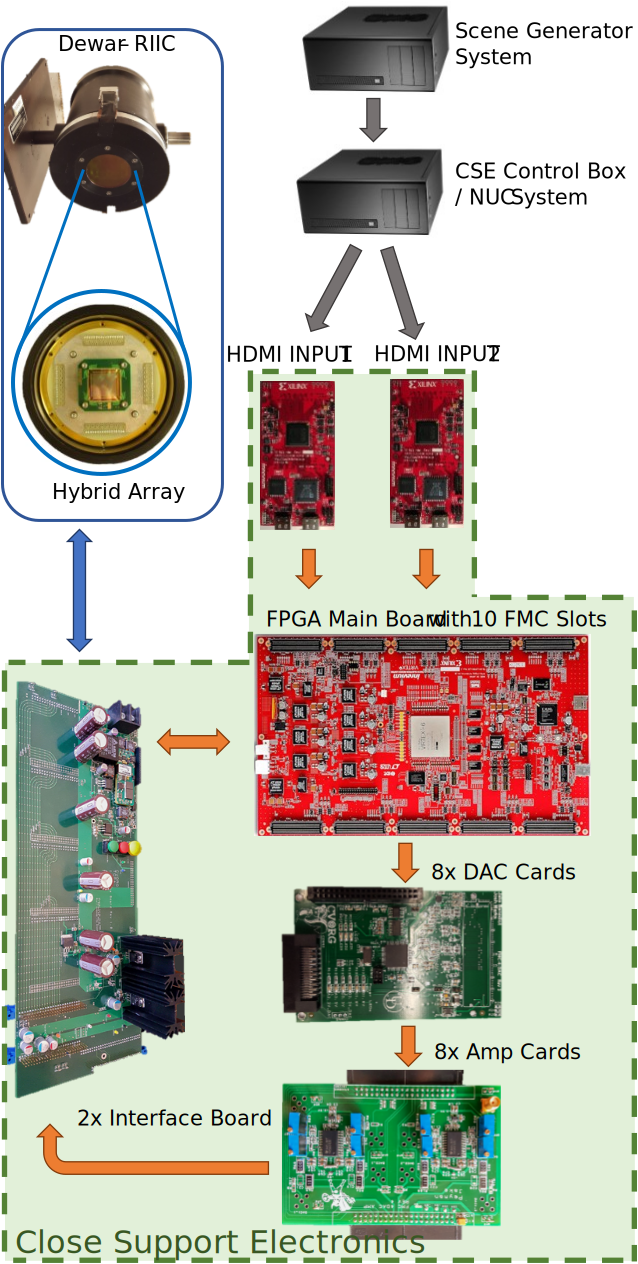
\includegraphics[width=0.65\textwidth]{fig/sleds_block.pdf}
        \caption{SLEDS System Block Diagram}
        \label{fig:sleds_block}
    \end{figure}

    Once enough data is buffered, the firmware will control the write process to drive the 8 DAC cards which each house 2 16-bit DAC integrated circuits per card, with each circuit consisting of 2 channels per DAC. Yielding 32 parallel channels with 512 total signals. Once the DAC process is done, the analog output of the 32 channels is then amplified and routed to the array through ribbon cables. Figure~\ref{fig:nessie_enclosure_internals} shows the components installed within a CSE with the ribbon cables shown in the top right. Additional control signals provided by the firmware and routed to the RIIC through these cables are discussed in Chapter~\ref{sec:array_Interleaved_write_process}. The specifics of the PDP firmware architectures write process are discussed in Chapter~\ref{chap:implementation}.

    \begin{figure}
        \centering
        \includegraphics[width=1.0\textwidth]{fig/nessie_enclosure_internals.jpg}
        \caption{CSE Internals}
        \label{fig:nessie_enclosure_internals}
    \end{figure}

\section{Communication Flow}

    Figure~\ref{fig:cse_comm_block} shows the internals of CSE communication. Communication for controlling the behavior of CSE is done through a daisy chained set of UART devices utilizing a reliable two way communication protocol called the CVORG protocol\footnote{Named after my research group at the University of Delaware.}. Without loss of generality, the protocol itself consist of commands to control various aspects of operation, such as, tripping an array, setting voltage limits, and configuring firmware operation. It also allows for information to be retrieved about current system configuration, as well as, operational errors. The destination of an operation is encoded as part of each command. Thus, commands not meant for a given component are forwarded along the chain.

    Memory mapped I/O between the frontend and backend firmware is controlled by the microblaze soft processor and used to control the underlying PDP firmware registers, as well as, program an array using Serial Peripheral Interface (SPI) (Not shown). The underlying details of the CVORG protocol itself are beyond the scope of this work and will not be discussed here. The details of command operations will be discussed in Chapter~\ref{sec:frontend_arch}. Additionally, SPI communication is also used to send data for LCD readout. Typically this includes voltage and current information, as well as, the results of power on sanity checks. Finally, the details of the processing performed on HDMI display data sent directly to the Backend Firmware as will be discussed in Chapter~\ref{sec:backend_arch}.

    \begin{figure}
        \centering
        \includegraphics[width=1.0\textwidth]{fig/cse_comm_block.pdf}
        \caption{CSE Internal Communication Block Diagram}
        \label{fig:cse_comm_block}
    \end{figure}

    Figures~\ref{fig:external_cse_comm_direct},~\ref{fig:external_cse_comm_half_indirect},~and~\ref{fig:external_cse_comm_indirect} show the details of external communication to a CSE in various configurations. In all configurations, a Low Pin Count (LPC) FPGA Mezzanine Card (FMC) connector provides the ability for various interfaces to be used to send data to the CSE, such as serial protocols or display based protocols over different types of hardware links. The FMC interface cards are responsible for retrieving the data over the link and formatting it in a manner that the internal CSE FPGA can decode. In practice, 24-bit pixel words and a data enable pin are utilized. In display protocol setups, a vertical sync signal is also utilized to reset pixels every display frame. As mentioned earlier in this section, current CSE setups utilize two HDMI FMC cards for input where the input for the top half of an array will be delivered over one cable and the bottom over the other. API communication on the other hand utilizes UART and the CVORG protocol.

    Figure~\ref{fig:external_cse_comm_direct} depicts direct communication in which formated scene data is sent directly to a CSE and system configuration is done directly by a scene generator. In this type of setup, the scene generator can monitor CSE operation directly, as well as, operate in either a closed or open loop type setup. This type of setup is desirable for minimizing end-to-end latency within an system for use cases where performance is paramount. For example, closed loop scenerios may feed recorded output imagery from an array back into the scene generator for in the loop analysis or in some cases subsequent frames may depend on the recorded results from prior frames.

    \begin{figure}
        \centering
        \includegraphics[width=1.0\textwidth]{fig/external_cse_comm_direct.pdf}
        \caption{CSE External Direct Communication Block Diagram}
        \label{fig:external_cse_comm_direct}
    \end{figure}

    Figure~\ref{fig:external_cse_comm_half_indirect} depicts indirect API communication in which system configuration is done through client APIs, and scene data is sent directly to a CSE. This type of setup is useful for situations where control over a CSE is needed but where API operation cannot be tightly coupled with a scene generator due to development costs, practical reasons, etc. In this setup, thin client API shims are provided to execute commands using remote procedure calls (RPC) which then are executed within a CSE operations box to communicate with the CSE. Similar to the direct setup, end-to-end latency is minimized by directly driving an array.

    \begin{figure}
        \centering
        \includegraphics[width=1.0\textwidth]{fig/external_cse_comm_half_indirect.pdf}
        \caption{CSE External Indirect API Communication Block Diagram}
        \label{fig:external_cse_comm_half_indirect}
    \end{figure}

    Figure~\ref{fig:external_cse_comm_indirect} depicts an indirect setup in which both API communication and scene data are sent to an intermediate CSE operations box. This type of setup is utilized in the event that data cannot be formatted directly for display on an array within a scene generator. It may also be utilized in cases where non-uniformity correction is performed externally from scene generation as shown in Figure~\ref{fig:sleds_block}. A third scenerio where this type of setup may be used is without a scene generator, where a CSE operation box could be used to characterize an array directly, as well as, to test and troubleshoot operations. Similarly, to the other indirect API communication setups, client API shims are provided to execute commands using remote procedure calls (RPC) which then are executed within a CSE operations box to communicate with the CSE.

    \begin{figure}[H]
        \centering
        \includegraphics[width=1.0\textwidth]{fig/external_cse_comm_indirect.pdf}
        \caption{CSE External Indirect API and Data Communication Block Diagram}
        \label{fig:external_cse_comm_indirect}
    \end{figure}

    While this chapter covered the flow of communication within and without a CSE, Chapter~\ref{chap:array_write_process} shifts focus to discuss the hardware details of an IRLED array's write process and the formatting of data sent to arrays.
